\documentclass[12pt,letterpaper]{article}

% Minimal package set: each supports content (equations, figures, citations,
% the data-availability URL); geometry only sets page margins.
\usepackage[margin=1in]{geometry}
\usepackage{amsmath}            % displayed equations
\usepackage{graphicx}          % figures
\usepackage{url}               % data-availability URL
\usepackage[superscript]{cite} % ACS-style superscript reference citations
\graphicspath{{figures/}}
\pagestyle{plain}

\begin{document}

% title block
\begin{center}
  {\LARGE\bfseries Structure--Activity Landscape Roughness Predicts Per-Compound QSAR Error Independently of the Applicability Domain\par}
  \vspace{1.2em}
  {\large Krishna Harish\textsuperscript{1}\par}
  \vspace{0.7em}
  {\itshape\textsuperscript{1}Elkins High School, Missouri City, Texas, United States\par}
  \vspace{0.5em}
  {*Email: krishnaharish2009@gmail.com\par}
\end{center}
\vspace{1em}

\begin{center}\textbf{Abstract}\end{center}
\noindent Machine-learning models of molecular potency fail systematically on activity cliffs, structurally similar molecules with large potency differences, yet give no warning when a prediction lands on one. The reliability tools in common use look the wrong way: applicability-domain and uncertainty methods flag extrapolation into sparse chemical space, but cliffs sit among close analogs, in the dense regions those methods treat as safe. We ask whether the error a model makes on a specific compound can instead be anticipated from the local roughness of the structure--activity landscape, measured from structure alone. On thirty bioactivity benchmarks, activity-free descriptors computable before any assay predict per-compound random-forest error on every target: neighborhood activity dispersion most strongly (median Spearman 0.28), while the pairwise density of the Structure--Activity Landscape Index flags labeled cliffs with a median area under the receiver-operating-characteristic curve of 0.69, and nearest-neighbor similarity, the basis of the applicability domain, points the opposite way. The signal survives control for the applicability domain in partial-correlation and mixed-effects analyses, so it is a distinct axis of reliability, not a proxy for data sparsity. The effects are modest but uniformly consistent, hold across three model classes and distance metrics, and replicate on solubility and lipophilicity benchmarks outside bioactivity. Conditioning a conformal predictor on this roughness, rather than on the applicability domain, holds 90\% interval coverage flat across the roughness range and restores it on activity cliffs, where unconditional intervals silently under-cover. A measure that uses the query's own activity tracks error more strongly (median Spearman 0.65) but is a mechanistic upper bound, not a usable signal, since it needs the very potency being predicted. The result is a model-agnostic, structure-only estimate of where a quantitative structure--activity relationship (QSAR) prediction should and should not be trusted.

\section*{Keywords}
activity cliffs; QSAR; structure--activity landscape; applicability domain; uncertainty quantification; machine-learning reliability

\section*{Introduction}

Quantitative structure--activity relationship (QSAR) modeling and, more recently, deep learning are routine tools for prioritizing compounds in drug discovery, used to predict potency, selectivity, and pharmacokinetic properties from chemical structure.\cite{vamathevan2019,walters2021} Almost all such models rest, implicitly or explicitly, on the molecular similarity principle: structurally similar molecules tend to exhibit similar properties.\cite{johnson1990} This assumption is what allows a model trained on known compounds to generalize to new ones, and it is embedded in the inductive biases of the most widely used representations and algorithms, from fingerprint-based nearest-neighbor and kernel methods to message-passing graph neural networks, all of which map similar structures to similar predictions.

Activity cliffs are the principled exception to this rule.\cite{maggiora2006,stumpfe2012} A cliff is a pair of structurally similar molecules whose potencies differ by orders of magnitude, a discontinuity in the structure--activity landscape that directly violates the similarity assumption. Cliffs are not rare curiosities; they are pervasive across medicinal-chemistry data sets and frequently mark precisely the structural transformations that matter most during optimization.\cite{cruzmonteagudo2014} Because they break the assumption on which prediction relies, cliffs are where models fail. A recent benchmark established this systematically: across 30 targets, machine-learning models, and deep neural networks in particular, predicted cliff compounds substantially less accurately than the rest, with descriptor-based methods outperforming graph- and sequence-based deep learning and no method reliably mastering cliffs.\cite{vantilborg2022,dablander2023} The practical consequence is a problem of trust: a model may issue a confident prediction for a compound that sits on a cliff, exactly where that prediction is least reliable. A modeler able to identify cliff-prone compounds in advance (from structure, before any assay) could flag unreliable predictions, triage compounds for experimental confirmation, and interpret model error.

Existing tools address adjacent but distinct questions. Roughness of the structure--activity landscape has been quantified at the level of an entire data set: the ROGI index\cite{aldeghi2022} and its representation-normalized successor,\cite{graff2023} together with earlier modelability indices such as MODI\cite{golbraikh2014} and SARI,\cite{peltason2007} return a single scalar that correlates with a model's overall error and answers whether a data set is hard to model. At the opposite granularity, the Structure--Activity Landscape Index (SALI)\cite{guha2008} quantifies the steepness of an individual pair of molecules. Neither resolves the question we pose, which specific compounds a model will mispredict, because one aggregates over the whole landscape and the other describes edges rather than compounds. Methods designed for per-compound reliability, namely applicability-domain analyses\cite{netzeva2005,sahigara2012} and uncertainty estimators such as ensemble variance and conformal prediction,\cite{norinder2014,hirschfeld2020} target a different failure mode: they measure how far a query lies from the training data and thereby flag extrapolation into sparsely sampled chemical space. Activity cliffs, however, occur in densely sampled regions, among close analogs, where applicability-domain methods report high confidence. To our knowledge, no per-compound, activity-free measure of local landscape roughness has been shown to predict QSAR error while being demonstrably distinct from the applicability domain.

Here we close that gap. We define a small family of local roughness functionals computed from a compound's nearest training neighbors: a similarity-weighted local Dirichlet energy and a Lipschitz aggregate that use the compound's own activity, and three activity-free measures (neighborhood activity dispersion, the pairwise-SALI density of the neighborhood, and a local H\"older regularity exponent) that do not. Using the 30-target MoleculeACE benchmark and its fixed splits, we evaluate whether these quantities predict the per-compound out-of-sample error of a random-forest model, and we test the result against applicability-domain and uncertainty baselines, a data-set-level roughness index, and a graph-convolutional model, across a range of neighborhood sizes and three distance metrics.

Our central result is that this gap closes with a measure that uses no activity information. An activity-free descriptor, the pairwise-SALI density of a compound's training neighbors, predicts per-compound random-forest error on all 30 targets and flags benchmark-labeled cliffs with useful accuracy, entirely from structure. This signal is distinct from the applicability domain: it survives partial-correlation and mixed-effects control for nearest-neighbor similarity and local density, and for cliffs the two notions are not merely separable but opposed, because applicability-domain similarity is built to warn about sparse regions whereas cliffs concentrate among close analogs. The relationship is general rather than an artifact of one benchmark or one learner; it holds across random forests, gradient boosting, and support-vector regression, is stable across neighborhood size and three distance metrics, and reproduces on two physicochemical benchmarks outside bioactivity. It is also actionable: used as the nonconformity scale of a conformal predictor, the descriptor produces 90\% prediction intervals that recover their coverage on activity cliffs, which standard and applicability-domain-scaled intervals do not. A second pair of descriptors that read the query compound's own activity correlate with error more strongly (a similarity-weighted local Dirichlet energy reaches a median Spearman of 0.65), but because they require the potency being predicted they bound what local geometry can explain rather than provide a signal a modeler could deploy. We are explicit throughout that the activity-free effect sizes are modest; their value is that they are consistent on every target and orthogonal to the reliability axes already in use. A graph-convolutional baseline, included only to characterize a standard message-passing model, loses to descriptors in smooth regions rather than at cliffs, where both fail comparably.

\section*{Computational Methods}

\subsection*{Benchmark data sets}

All analyses used the MoleculeACE benchmark,\cite{vantilborg2022} a curated collection of bioactivity data for 30 macromolecular targets drawn from ChEMBL v29,\cite{gaulton2012} comprising 48.7K measurements (35.6K unique structures) across 23 inhibition-constant ($K_i$) and 7 half-maximal effective concentration (EC$_{50}$) end points. For each target the regression target $y$ is the base-10 logarithm of potency ($-\log_{10}$ of the activity in nM; equivalently p$K_i$ or pEC$_{50}$ up to an additive constant), so that one unit corresponds to one order of magnitude in potency. Across the test compounds analyzed here $y$ spanned $-5.0$ to $2.0$ (mean $-1.8$).

Activity-cliff annotations and train/test partitions were taken unchanged from the benchmark to ensure that our per-compound error estimates are directly comparable to the published results. Following van Tilborg et al.,\cite{vantilborg2022} a pair of compounds was labeled an activity cliff when the two molecules differed by more than 10-fold in potency ($\Delta g > 1$) and were structurally similar by at least one of three complementary measures: substructure similarity (Tanimoto coefficient on extended-connectivity fingerprints), scaffold similarity (Tanimoto coefficient on Bemis--Murcko scaffold fingerprints), or SMILES similarity (scaled Levenshtein distance), with any of the three exceeding 0.9. A molecule was designated a cliff compound if it participated in at least one such pair. Train/test splits were those distributed with the benchmark, obtained by spectral clustering of each data set on extended-connectivity fingerprints followed by stratified 80/20 partitioning within clusters. The resulting test sets contained 126--733 compounds per target (9{,}802 in total); the fraction of cliff compounds ranged from 9\% to 54\% across targets (38.7\% overall). For external validation beyond bioactivity, two MoleculeNet physicochemical regression benchmarks were additionally analyzed: aqueous solubility (ESOL; 1{,}128 compounds with measured log solubility\cite{delaney2004}) and lipophilicity (4{,}200 compounds with experimental $\log D$\cite{wu2018}). Lacking a distributed split, these were partitioned 80/20 by a Bemis--Murcko scaffold split,\cite{bemis1996} assigning whole scaffold groups to the training set in order of decreasing frequency.

\subsection*{Molecular representations and distance metrics}

Unless stated otherwise, molecules were represented by 2{,}048-bit extended-connectivity fingerprints of radius 2 (ECFP4\cite{rogers2010}) computed with RDKit, and the distance between two molecules $i$ and $j$ was defined as $d_{ij} = 1 - T_{ij}$, where $T_{ij}$ is the Tanimoto coefficient; the corresponding similarity is $s_{ij} = T_{ij}$. For robustness analyses two further representations were used: 2{,}048-bit ECFP6 fingerprints (radius 3) under the same Tanimoto distance, and a standardized 12-descriptor physicochemical vector (molecular weight, calculated logP, topological polar surface area, hydrogen-bond donor and acceptor counts, rotatable-bond count, aromatic-ring count, fraction of $sp^3$ carbons, heavy-atom count, ring count, heteroatom count, and molar refractivity) under Euclidean distance, with each descriptor standardized to zero mean and unit variance using training-set statistics.

For every test molecule $i$, its $k$ nearest neighbors $N_k(i)$ were identified among the \textbf{training} compounds under the chosen distance, so that all neighbor-derived quantities for a held-out molecule depend only on the training data and, where indicated, on that molecule's own activity. The default neighborhood size was $k = 10$.

\subsection*{Local landscape-roughness descriptors}

Two descriptors quantify the steepness of the structure--activity landscape in the immediate vicinity of a molecule and use the molecule's own activity $y_i$; we refer to these as \emph{landscape} descriptors. The first is a similarity-weighted local Dirichlet energy, defined as
\begin{equation}
R_D(i) = \frac{\sum_{j \in N_k(i)} s_{ij}\,(y_i - y_j)^2}{\sum_{j \in N_k(i)} s_{ij}}
\end{equation}
i.e., the similarity-weighted mean squared activity gap between $i$ and its neighbors; it is the discrete analogue of the squared gradient of the activity function evaluated at $i$. The second is a local Lipschitz constant, an aggregation of the pairwise SALI\cite{guha2008},
\begin{equation}
R_L(i) = \max_{j \in N_k(i)} \frac{|y_i - y_j|}{\max(1 - s_{ij},\,\varepsilon)}
\end{equation}
with $\varepsilon = 10^{-3}$ to bound the denominator for near-identical pairs.

\subsection*{Activity-free (a priori) roughness descriptors}

Three descriptors estimate local roughness \textbf{without} reference to the query molecule's activity, and are therefore computable before any potency is known; we refer to these as \emph{a priori} descriptors. The neighborhood activity dispersion,
\begin{equation}
D(i) = \operatorname{std}\{\, y_j : j \in N_k(i) \,\}
\end{equation}
measures the spread of activities among the query's training neighbors. The pairwise-SALI density summarizes the steepness of the landscape \emph{within} the neighbor set,
\begin{equation}
S_{\max}(i) = \max_{a,b \in N_k(i)} \frac{|y_a - y_b|}{\max(1 - s_{ab},\,\varepsilon)}
\end{equation}
with $S_{\mathrm{mean}}(i)$ the mean over the same neighbor set, using only neighbor activities and neighbor-to-neighbor similarities. Finally, a local H\"older (regularity) exponent was estimated over the $K_H = 25$ nearest training neighbors by ordinary-least-squares fitting of $\log|y_a - y_b| = \alpha \log d_{ab} + c$ across all neighbor pairs $(a, b)$; the slope $\alpha$ is a local estimate of the activity function's H\"older regularity, with smaller $\alpha$ indicating rougher behavior.

\subsection*{Baseline measures}

Three families of established measures were computed for comparison. \emph{Applicability-domain} measures characterize a molecule's proximity to the training data: the nearest-neighbor similarity $s_{\mathrm{NN}}(i) = \max_j s_{ij}$ over the training set, and the local density, the mean similarity over $N_k(i)$. An \emph{uncertainty} baseline was obtained from the random-forest predictor as the variance of the individual tree predictions for each test molecule. A \emph{global-roughness} baseline was obtained with the ROGI index,\cite{aldeghi2022} a single dataset-level scalar that quantifies structure--property surface roughness through the loss of property dispersion under progressive coarse-graining; ROGI was computed per data set on the full activity distribution using the reference implementation, which also provides the SARI and (R)MODI modelability indices.

\subsection*{Predictive models}

A descriptor-based and a graph-based regressor were trained per target on the official training split and evaluated on the official test split; the per-compound out-of-sample error was $e_i = |\hat{y}_i - y_i|$.

The descriptor model was a random forest\cite{breiman2001} as implemented in scikit-learn, with 200 trees and $\sqrt{p}$ features considered per split, fit on 2{,}048-bit ECFP4 features. Per-compound predictive variance was taken as the variance across the 200 tree predictions.

The graph model was a Graph Isomorphism Network (GIN\cite{xu2019}) implemented in PyTorch. Each atom was described by a 16-dimensional feature vector (one-hot atomic number over C, N, O, F, P, S, Cl, Br, I, other, degree, formal charge, aromaticity flag, total hydrogen count, and ring-membership flag). Three GIN-0 layers with hidden width 64 propagated information according to $\mathbf{H}^{(l+1)} = \mathrm{MLP}^{(l)}(\mathbf{H}^{(l)} + \mathbf{A}\,\mathbf{H}^{(l)})$, where $\mathbf{A}$ is the bond adjacency matrix; the graph embedding was the sum over layers of the mean of the node embeddings, followed by a two-layer multilayer-perceptron head. Models were trained with Adam (learning rate $10^{-3}$) to minimize the mean squared error on standardized targets. Two training regimens were compared. The first used a fixed schedule of 60 epochs. The second (``tuned'') held out 10\% of the training set for validation, trained for up to 150 epochs with learning-rate reduction on plateau and best-checkpoint early stopping (patience 20), and used size-bucketed mini-batches of 128 to minimize padding. Per-compound test errors were computed as for the random forest. For the model-class generality analysis, two additional regressors were trained on the same ECFP4 features and splits (a histogram gradient-boosting regressor and a support-vector regressor (SVR) with a radial-basis-function (RBF) kernel, $C = 10$), each yielding per-compound test errors in the same way.

\subsection*{Statistical analysis}

The primary analysis quantified, for each target, the Spearman rank correlation between a descriptor and the per-compound random-forest error, then aggregated the 30 coefficients as the median and interquartile range, reporting the fraction of targets with the expected sign and a two-sided Wilcoxon signed-rank test of the coefficients against zero; $p$ values across descriptors were adjusted by the Benjamini--Hochberg false-discovery-rate (FDR) procedure.\cite{benjamini1995} To test whether roughness is distinguishable from the applicability domain, partial Spearman correlations were computed per target by rank-transforming the descriptor, the error, and the control variables (nearest-neighbor similarity and local density), residualizing the descriptor and the error on the controls by ordinary least squares, and correlating the residuals; the resulting coefficients were aggregated as above. As a confound-controlled confirmation, a linear mixed-effects model (statsmodels) regressed within-target standardized error on within-target standardized roughness, with nearest-neighbor similarity, local density, and heavy-atom count as fixed-effect covariates and a per-target random intercept. The ability of a priori descriptors to flag benchmark-labeled cliffs was assessed by the per-target area under the receiver-operating-characteristic curve (AUC), aggregated as the median and range. All correlation and classification analyses were repeated for $k \in \{5, 10, 15, 20, 30\}$ and for the three distance metrics described above to assess robustness. Operational utility was assessed by an enrichment analysis: within each target, compounds were ranked by a risk score (local roughness; the negative nearest-neighbor similarity, representing the applicability domain in its standard orientation; or the random-forest tree variance, representing uncertainty), and the fraction of positives captured within the top $f\%$ was computed and averaged across targets, with positives defined either as top-quartile-error compounds or as labeled activity cliffs.

To test whether the descriptors translate into calibrated prediction intervals, we built inductive (split) conformal\cite{norinder2014,papadopoulos2002} 90\% intervals from the held-out per-compound residuals, asking not how to normalize a conformal predictor but which per-compound variable it should be conditioned on. Within each target the test compounds were split at random into equal calibration and evaluation halves. We compared an unconditional predictor (nonconformity score $|\hat{y}_i - y_i|$, constant-width intervals) against two standard ways of making coverage conditional on a per-compound difficulty estimate: a locally-weighted (normalized) score $|\hat{y}_i - y_i| / \sigma(x_i)$,\cite{papadopoulos2011} and a Mondrian scheme\cite{bostrom2020} that stratifies the calibration set into quintiles of a conditioning variable and calibrates within each. For both, the conditioning variable was an activity-free roughness (the pairwise-SALI density) or, for comparison, the applicability domain ($1 - s_{\mathrm{NN}}$); every variant retains the finite-sample marginal coverage guarantee at $1 - \alpha = 0.9$. We report marginal, activity-cliff, and non-cliff coverage, interval width, and coverage as a function of local-roughness quantile, averaged over 50 random calibration/evaluation splits and aggregated as the median across targets.

\subsection*{Software and data availability}

Analyses used Python 3.12 with RDKit (2026.03), scikit-learn (1.8), PyTorch (2.12), statsmodels, SciPy, the rogi package, NumPy, and pandas. The MoleculeACE benchmark data, activity-cliff labels, and train/test splits were obtained from the MoleculeACE Python package. All code required to reproduce the descriptors, models, statistics, and figures is available at \url{https://github.com/krishnatheaverage/qsar-landscape-roughness}.

\section*{Results and Discussion}

\subsection*{Activity cliffs concentrate prediction error}

Across the 30 benchmarks, activity-cliff compounds were predicted markedly less accurately than non-cliff compounds by the random forest, reproducing on our pipeline the observation that motivates the benchmark. The mean absolute test error was 0.62 log units for cliff compounds versus 0.46 for non-cliff compounds, a median per-target ratio of 1.35, and cliff error exceeded non-cliff error in 29 of the 30 targets (Wilcoxon signed-rank $p = 3.7 \times 10^{-9}$). Cliffs are thus a generic and reproducible failure mode rather than an artifact of any single data set, and the remainder of this work asks whether that failure can be anticipated from the geometry of the local landscape.

\subsection*{Structure-only roughness predicts per-compound error}

We treated each target as an independent replicate and asked the question a modeler actually faces: can a per-compound quantity computed from structure alone, before any activity is in hand, predict which test compounds the random forest will get wrong? We summarize the answer as the distribution of per-target Spearman correlations across the 30 data sets (Figure~\ref{fig:main}A). It can. The activity-free neighborhood dispersion $D$, the spread of a compound's training neighbors' activities, was positively correlated with per-compound error on all 30 targets (median Spearman $\rho = 0.28$, false-discovery-rate-adjusted $p = 2.7 \times 10^{-9}$), and the pairwise-SALI density of the neighborhood behaved likewise (median $\rho = 0.16$, positive on all 30). These correlations are modest, and we treat them as modest throughout; their importance is that they are consistent in sign on every target and that they beat the reliability signals already in use. Both exceeded the two applicability-domain baselines, nearest-neighbor similarity and local density (median $\rho \approx 0.18$--$0.19$), and the only baseline that predicted error more strongly, the random-forest tree variance (median $\rho = 0.36$), is not a structural quantity at all but a property of the fitted ensemble, available only after training and prediction. That a purely structural measure tracks per-compound error on every target is the central observation of this work: cliff-prone regions announce themselves before any potency is measured.

\begin{figure}[htbp]
\centering
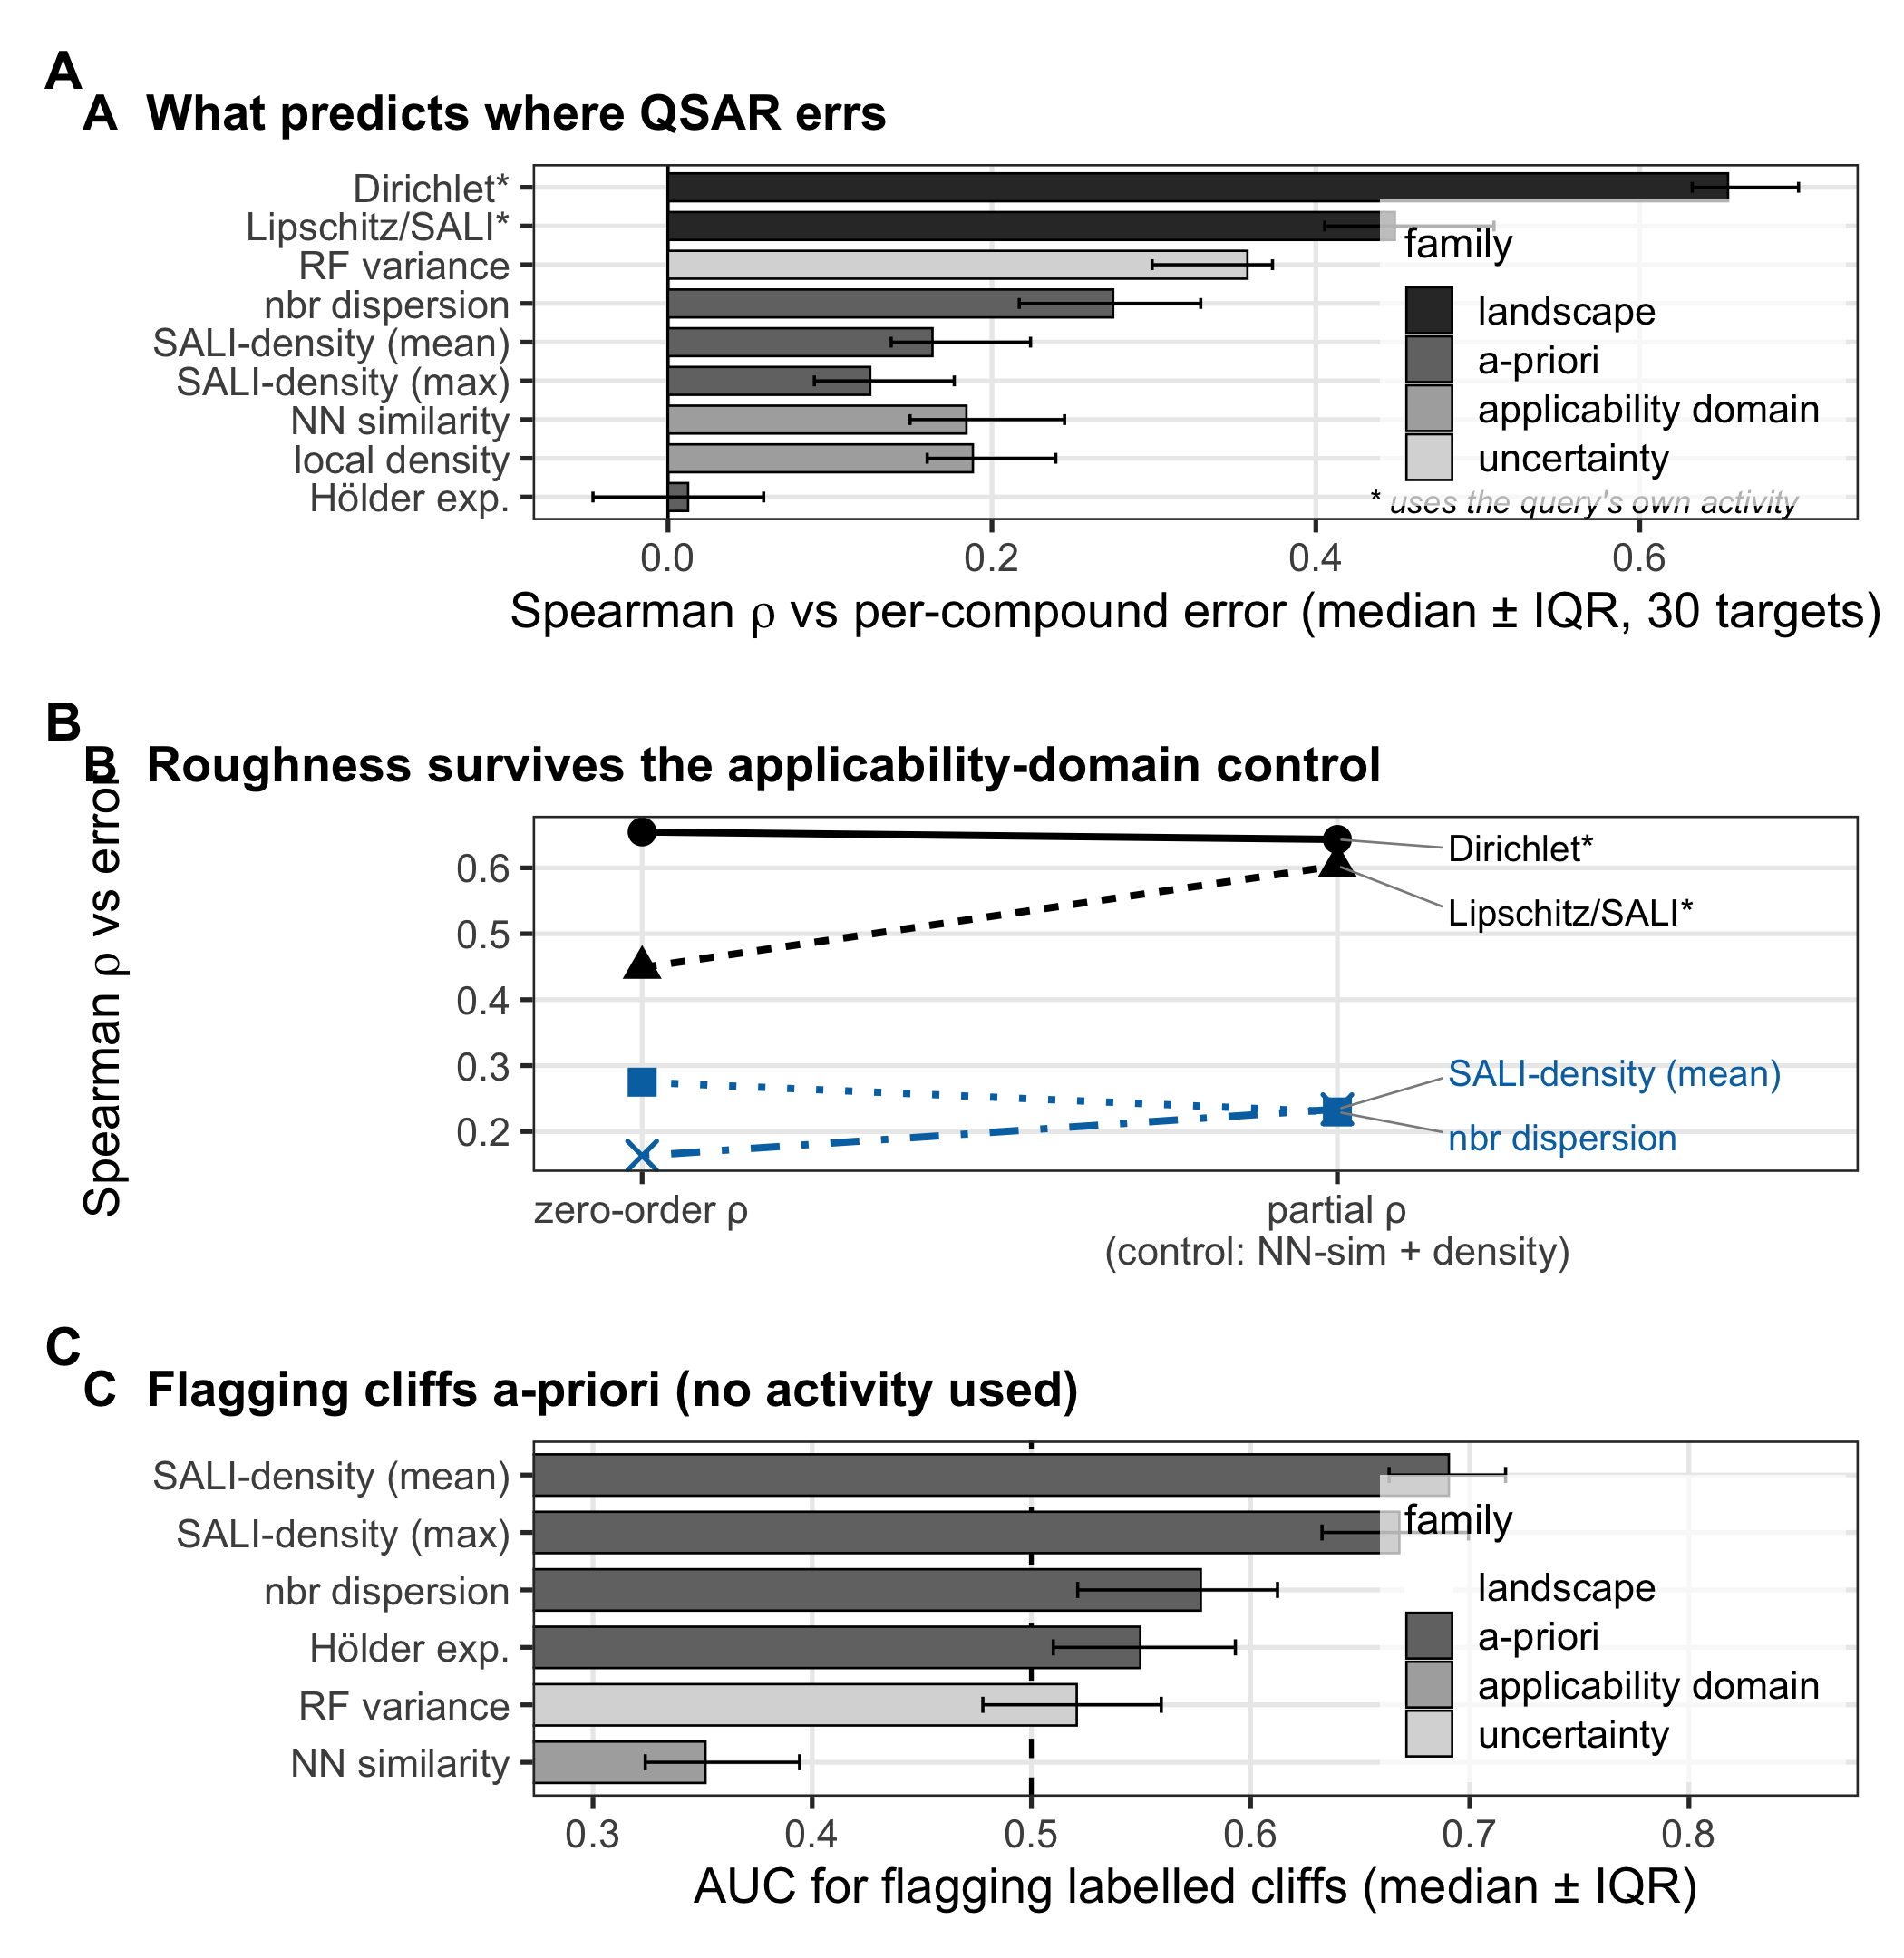
\includegraphics[width=\linewidth]{figure1_main.png}
\caption{Local structure--activity landscape roughness predicts per-compound QSAR error across 30 bioactivity targets. (A) Median Spearman correlation between each descriptor and per-compound random-forest error (median $\pm$ interquartile range over 30 targets); landscape descriptors (red) use the query compound's own activity, the activity-free descriptors (blue) do not, and applicability-domain (gray) and uncertainty (green) baselines are shown for reference. (B) Zero-order versus applicability-domain-controlled partial correlations; the relationship is retained or strengthened under control. (C) Area under the ROC curve for flagging benchmark-labeled activity cliffs from activity-free descriptors; nearest-neighbor similarity (gray) falls below 0.5 in the extrapolation orientation because cliffs cluster among close analogs.}
\label{fig:main}
\end{figure}

The descriptors that incorporate the query compound's own activity set an upper bound on this effect rather than supplying a stronger version of it. The similarity-weighted local Dirichlet energy $R_D$ correlated with error far more strongly (median $\rho = 0.65$, interquartile range 0.59--0.68, positive on all 30 targets; FDR-adjusted $p = 2.7 \times 10^{-9}$), and the Lipschitz/SALI aggregate similarly (median $\rho = 0.45$). That strength is in part mechanistic and in part definitional: a tree ensemble interpolates the activities of nearby training molecules, so a compound whose measured activity departs sharply from its neighbors' is necessarily mispredicted, and $R_D$ is built from precisely that departure. Computing it requires the potency one is trying to predict, so $\rho = 0.65$ should be read as how much of the per-compound error local geometry can explain in principle, an upper bound, not as a number available before assay. The rest of this work concerns the activity-free descriptors, which can be computed without it.

\subsection*{Roughness is distinct from the applicability domain}

The neighborhood-dispersion result could in principle reflect nothing more than data sparsity: compounds in poorly sampled regions are both harder to predict and more likely to have heterogeneous neighbors. The decisive test is therefore whether roughness predicts error \emph{after} the applicability domain is controlled. Partial Spearman correlations, removing the rank contribution of nearest-neighbor similarity and local density, left the roughness signal intact (Figure~\ref{fig:main}B). The landscape Dirichlet energy retained essentially all of its association ($0.65 \rightarrow 0.64$), and the activity-free descriptors held or strengthened: neighborhood dispersion fell only modestly ($0.28 \rightarrow 0.23$) and the pairwise-SALI density rose ($0.16 \rightarrow 0.23$). The strengthening of several partial correlations indicates that the applicability-domain variables act as mild suppressors rather than as the underlying cause. A linear mixed-effects model reached the same conclusion under simultaneous control of nearest-neighbor similarity, local density, molecular size, and a per-target random intercept: standardized neighborhood dispersion carried a coefficient of $+0.26$ (standard deviations of error per standard deviation of dispersion; $p = 5 \times 10^{-143}$), the pairwise-SALI density $+0.13$ ($p = 1 \times 10^{-41}$), and the landscape Dirichlet energy $+0.73$. Local landscape roughness is thus a distinct axis of predictability, not a re-expression of distance to the training set; this is the central claim of this work.

\subsection*{Generality across model classes}

Because per-compound error was measured primarily with a random forest, we asked whether the relationship is a property of the landscape or of that particular algorithm. Repeating the analysis with two further model classes trained on the same fingerprints and splits (gradient-boosted trees and a radial-basis-function support-vector regressor) gave the same picture (Table~\ref{tab:models}). The landscape Dirichlet energy correlated with per-compound error at a median Spearman $\rho$ of 0.65, 0.58, and 0.55 for the random forest, gradient boosting, and support-vector regressor, respectively; the activity-free neighborhood dispersion at 0.28, 0.25, and 0.24; and the partial correlation, after controlling for the applicability domain, at 0.23, 0.21, and 0.18. The signal is therefore model-agnostic: it tracks where the structure--activity landscape is locally rough, not an idiosyncrasy of a single learner.

\begin{table}[htbp]
\caption{Median Spearman correlation (across 30 targets) between local roughness and per-compound error for three model classes. The final column is the neighborhood-dispersion correlation after controlling for the applicability domain.}
\label{tab:models}
\centering
\begin{tabular}{lccc}
\hline
Model & Dirichlet (landscape) & Nbr.\ dispersion (activity-free) & Nbr.\ dispersion $\mid$ AD \\
\hline
Random forest & 0.65 & 0.28 & 0.23 \\
Gradient boosting & 0.58 & 0.25 & 0.21 \\
SVR (RBF) & 0.55 & 0.24 & 0.18 \\
\hline
\end{tabular}
\end{table}

\subsection*{Activity-free flagging of cliff-prone compounds}

If roughness anticipates error independently of the applicability domain, the activity-free descriptors should also flag the benchmark's labeled activity cliffs, and they do, with the caveat that the simplest descriptor is the weakest (Figure~\ref{fig:main}C). The pairwise-SALI density identified cliff compounds with a median per-target ROC-AUC of 0.69 (max-pooled variant 0.67), substantially above the neighborhood dispersion (0.58) and the random-forest uncertainty (0.52, indistinguishable from chance). The advantage of the SALI-density descriptors is interpretable: a query embedded among training analogs that themselves form a steep micro-landscape is far more likely to lie on a cliff than one whose neighbors merely span a wide activity range.

A complementary and initially counterintuitive observation concerns the applicability domain itself. Nearest-neighbor similarity, used directly, identified cliff compounds with a median AUC of 0.65, because cliffs occur preferentially among compounds with very close training analogs, as their definition (high similarity, large potency difference) requires. The implication is pointed: classical applicability-domain reasoning, which flags low-similarity extrapolation compounds as unreliable, is oriented exactly backward for cliffs, reassuring the modeler about the dense, high-similarity regions where cliffs in fact concentrate (the same variable, oriented toward extrapolation risk, gives an AUC of 0.35). Roughness and applicability domain are therefore not merely statistically separable but conceptually opposed for this failure mode.

Not every roughness construct succeeded. The local H\"older regularity exponent, estimated from the log--log scaling of activity differences with distance over each neighborhood, showed no association with error (median $\rho = 0.01$; FDR-adjusted $p = 0.61$) and no useful cliff-flagging ability (AUC 0.55). We attribute this to the instability of a two-parameter scaling fit over the small, discretely sampled neighborhoods available per compound, and report it as a negative result; the practical signal resides in the dispersion- and SALI-based descriptors.

\subsection*{Operational value: triaging unreliable predictions}

The correlations above translate into a concrete triage benefit, and clarify where roughness is and is not the right signal (Figure~\ref{fig:triage}). When the goal is to recover the highest-error predictions in general, the model's own ensemble uncertainty is the strongest single flag: flagging the top 20\% of compounds by random-forest tree variance recovers 38\% of the top-quartile-error compounds (a 1.9-fold enrichment over random), versus 33\% for roughness and 32\% for the applicability domain (Figure~\ref{fig:triage}A). The picture inverts for activity cliffs specifically (Figure~\ref{fig:triage}B). Flagging the top 20\% by roughness (pairwise-SALI density) recovers 33\% of labeled cliffs, a 1.6-fold enrichment, whereas ensemble uncertainty performs no better than random (1.0-fold) and the applicability domain is actively counterproductive (0.45-fold, worse than random, again because cliffs cluster among close analogs that the applicability domain deems safe). Roughness is therefore not a universal replacement for uncertainty estimation; its distinct value is that it captures the cliff failure mode that the standard reliability signals miss or invert.

\begin{figure}[htbp]
\centering
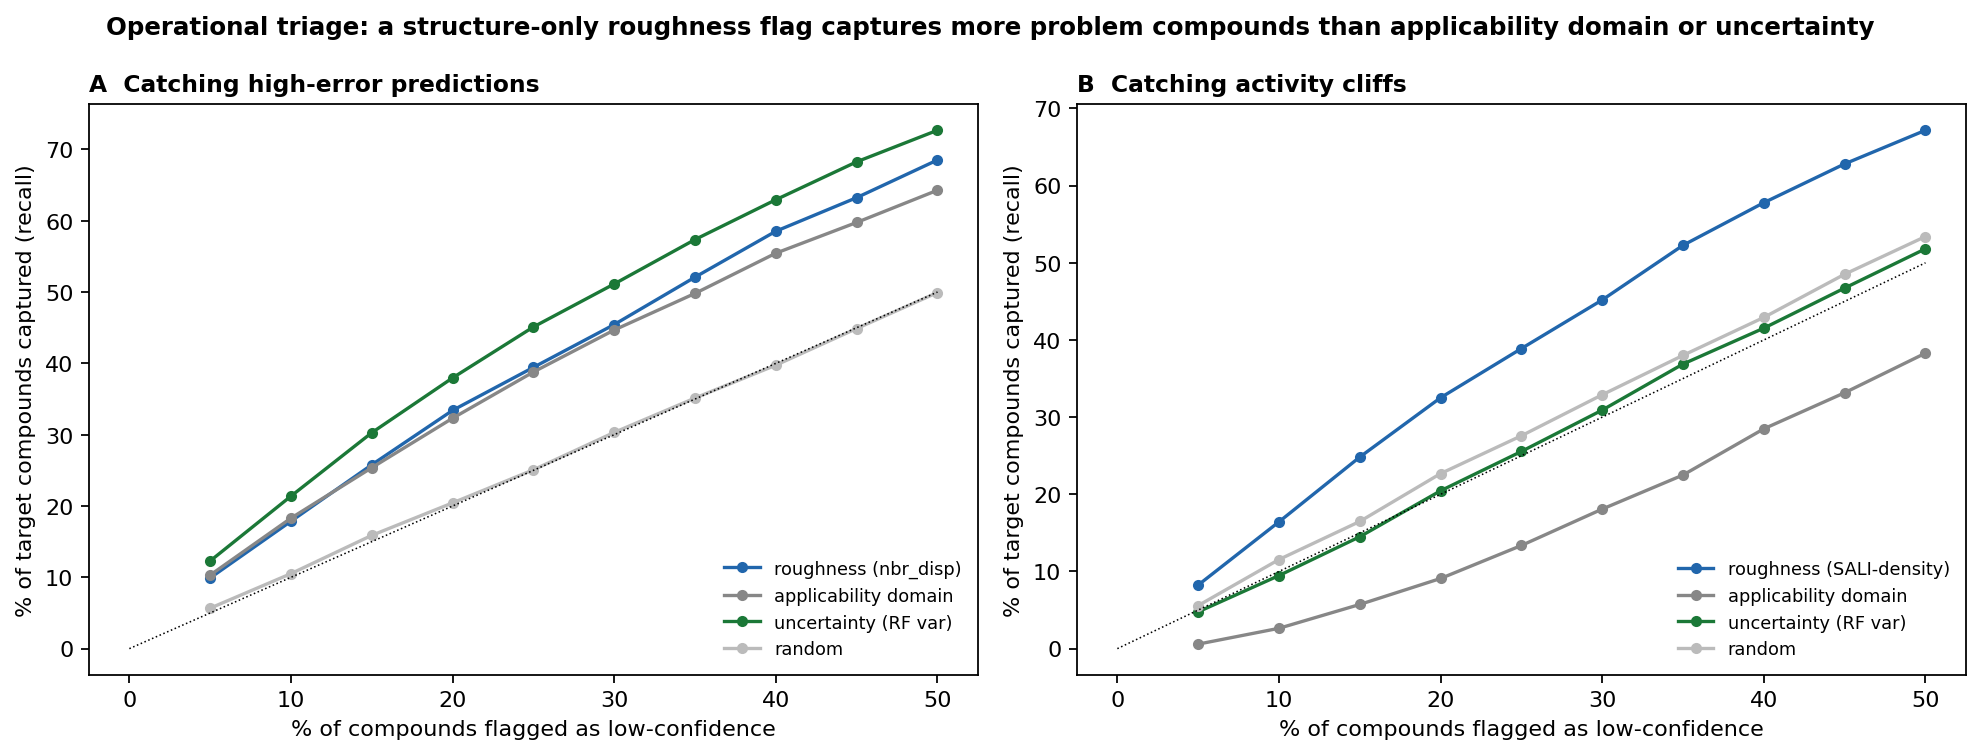
\includegraphics[width=\linewidth]{figure5_enrichment.png}
\caption{Operational triage value of a structure-only roughness flag. Fraction of (A) high-error predictions (top-quartile per-compound error) and (B) labeled activity cliffs recovered as a function of the percentage of compounds flagged as low-confidence, averaged over 30 targets, ranking by roughness (blue), the applicability domain in its standard orientation (gray), random-forest tree variance (green), or at random (dotted).}
\label{fig:triage}
\end{figure}

\subsection*{Robustness to neighborhood size and distance metric}

To establish that these relationships do not depend on arbitrary modeling choices, the per-target and partial correlations were recomputed across five neighborhood sizes ($k = 5$--30) and three distance definitions: Tanimoto similarity over ECFP4 and ECFP6 fingerprints and Euclidean distance in a standardized twelve-descriptor physicochemical space (Figure~\ref{fig:robust}). The relationship was stable throughout. Under ECFP4, a uniform-weight variant of the landscape roughness correlated with error at a median $\rho$ of 0.64 at $k = 5$, declining gently to 0.59 at $k = 30$, while neighborhood dispersion ranged from 0.27 to 0.22; ECFP6 yielded nearly identical values, indicating no dependence on fingerprint radius. In the lower-dimensional descriptor space the correlations attenuated ($\rho \approx 0.46$ and 0.15, respectively) but remained positive on all 30 targets, as expected for a representation that resolves structural neighborhoods more coarsely. Critically, the partial correlation controlling for nearest-neighbor distance and local density remained positive in all fifteen $k$--metric combinations. The signal is therefore not an artifact of any single similarity definition or neighborhood radius, and small neighborhoods ($k = 5$--10) are preferable.

\begin{figure}[htbp]
\centering
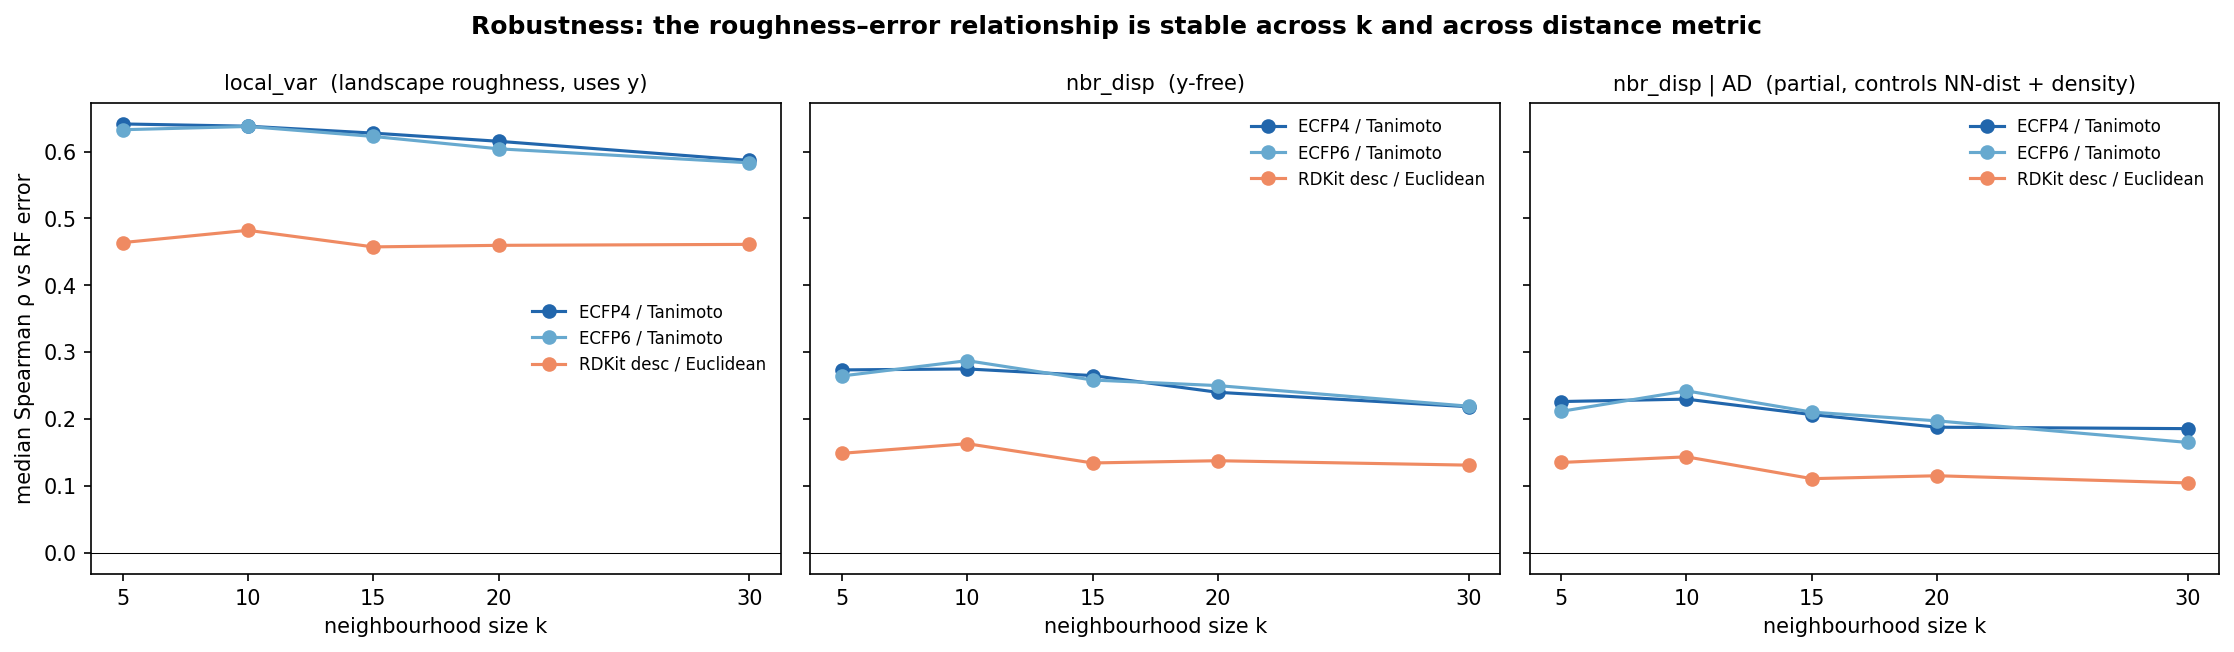
\includegraphics[width=\linewidth]{robustness_figure.png}
\caption{Stability of the roughness--error relationship across neighborhood size $k$ and molecular distance metric. Median Spearman correlation over 30 targets between per-compound random-forest error and (left) a landscape roughness measure, (center) the activity-free neighborhood dispersion, and (right) the neighborhood dispersion after controlling for the applicability domain, for ECFP4/Tanimoto, ECFP6/Tanimoto, and a 12-descriptor Euclidean representation.}
\label{fig:robust}
\end{figure}

\subsection*{External validation beyond bioactivity}

To test whether the relationship generalizes beyond the bioactivity setting in which it was developed, we applied the identical pipeline to two MoleculeNet physicochemical regression benchmarks, aqueous solubility (ESOL\cite{delaney2004}) and lipophilicity ($\log D$\cite{wu2018}), using scaffold splits\cite{bemis1996} rather than the bioactivity-specific partitions (Figure~\ref{fig:crossdomain}). The central result reproduced. Landscape roughness predicted the per-compound random-forest error on both tasks (Spearman $\rho = 0.60$ for solubility and 0.67 for lipophilicity) and retained essentially all of that association after the applicability domain was controlled (partial $\rho = 0.60$ and 0.64), closely matching the bioactivity value (0.65). The activity-free neighborhood dispersion also transferred, predicting error on both tasks ($\rho = 0.17$ and 0.20) and surviving the applicability-domain control on solubility (partial $\rho = 0.19$) though only weakly on lipophilicity (0.07), consistent with the modest and somewhat target-dependent magnitude of the activity-free signal observed throughout. Local landscape roughness therefore reflects a property of structure--activity and structure--property landscapes in general, rather than an idiosyncrasy of protein-binding data.

\begin{figure}[htbp]
\centering
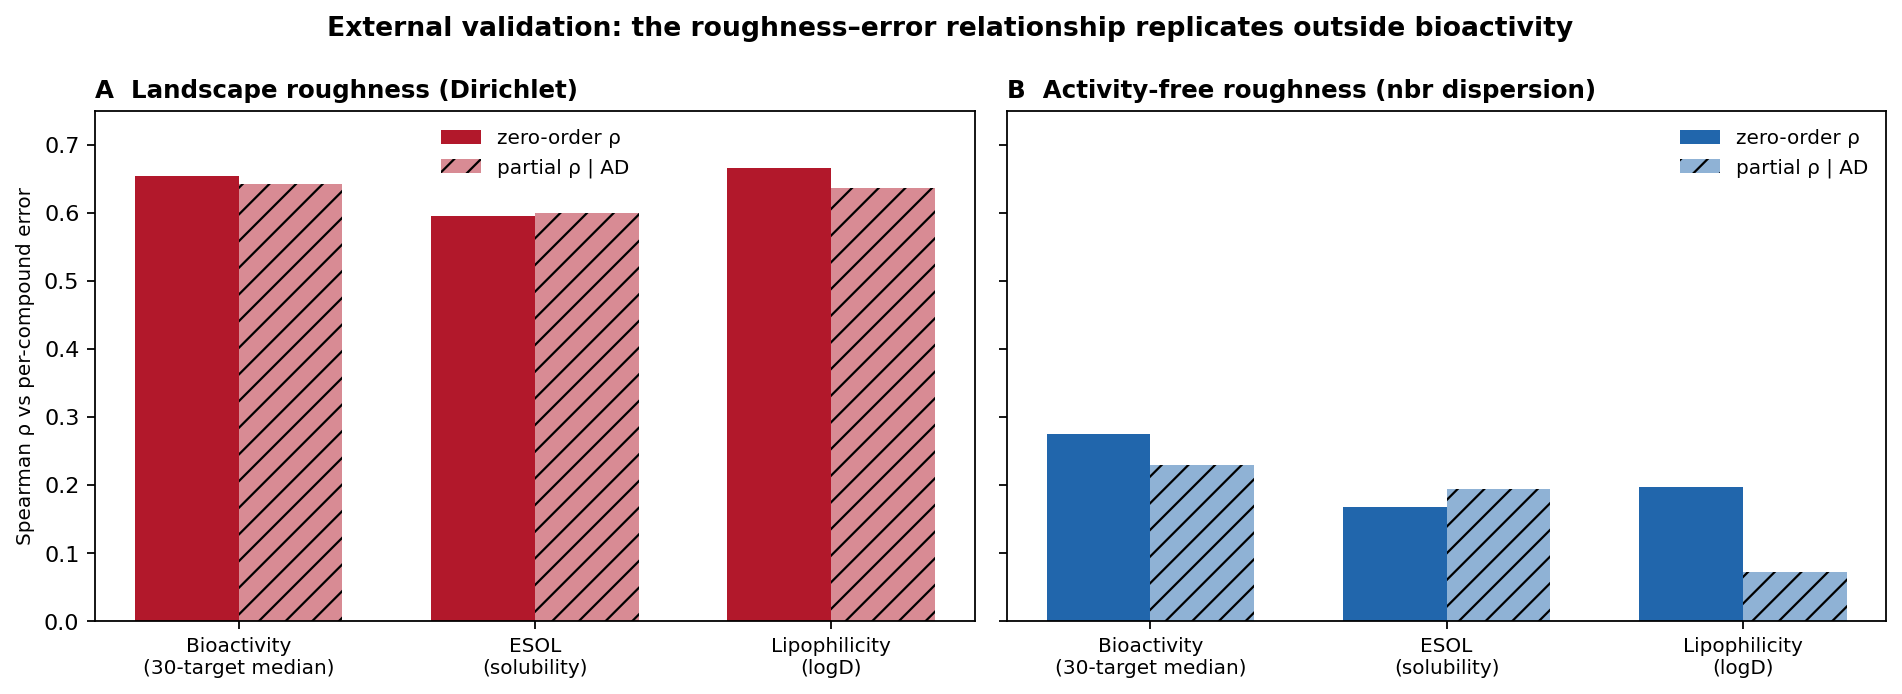
\includegraphics[width=\linewidth]{figure4_crossdomain.png}
\caption{External validation on physicochemical regression benchmarks. Zero-order and applicability-domain-controlled (partial) Spearman correlations between roughness and per-compound error for (A) the landscape Dirichlet energy and (B) the activity-free neighborhood dispersion, for the 30-target bioactivity median and for aqueous solubility (ESOL) and lipophilicity (logD).}
\label{fig:crossdomain}
\end{figure}

\subsection*{Where a graph-convolutional model underperforms}

We include a graph-convolutional model only to characterize where a standard message-passing baseline, not a tuned state-of-the-art network, gains or loses against descriptors; the comparison speaks to the behavior of a common baseline, not to the deep-learning ceiling. Consistent with prior benchmarking, the message-passing network produced higher mean absolute error (MAE) than the random forest on all 30 targets (0.71 versus 0.52 log units overall). Resolving this gap by local roughness revealed a counterintuitive pattern (Figure~\ref{fig:gnn}): the network's disadvantage was largest in the smoothest quartile of chemical space (mean error excess 0.25 log units) and smallest in the roughest quartile (0.13), and the per-compound error excess correlated negatively with roughness across targets (median Spearman $\rho = -0.07$, $p < 10^{-4}$); equivalently, the network's deficit on labeled cliffs (0.16) was smaller than on non-cliff compounds (0.21). Retraining the network with a held-out validation set, learning-rate scheduling, and best-checkpoint early stopping did not systematically reduce error (mean MAE 0.74; lower than the fixed-schedule model on only 10 of 30 targets), and both regimens reproduced the same roughness ordering. We therefore read the familiar ``descriptors outperform graph networks'' result on these data as reflecting an advantage concentrated in smooth, well-sampled regions rather than superior treatment of activity cliffs, where both model classes failed comparably. As a limitation, neither network was competitive with the descriptor model in absolute terms and architecture optimization was outside the scope of this study; this comparison characterizes standard graph-convolutional baselines rather than the deep-learning ceiling, and we present it as a supporting observation only.

\begin{figure}[htbp]
\centering
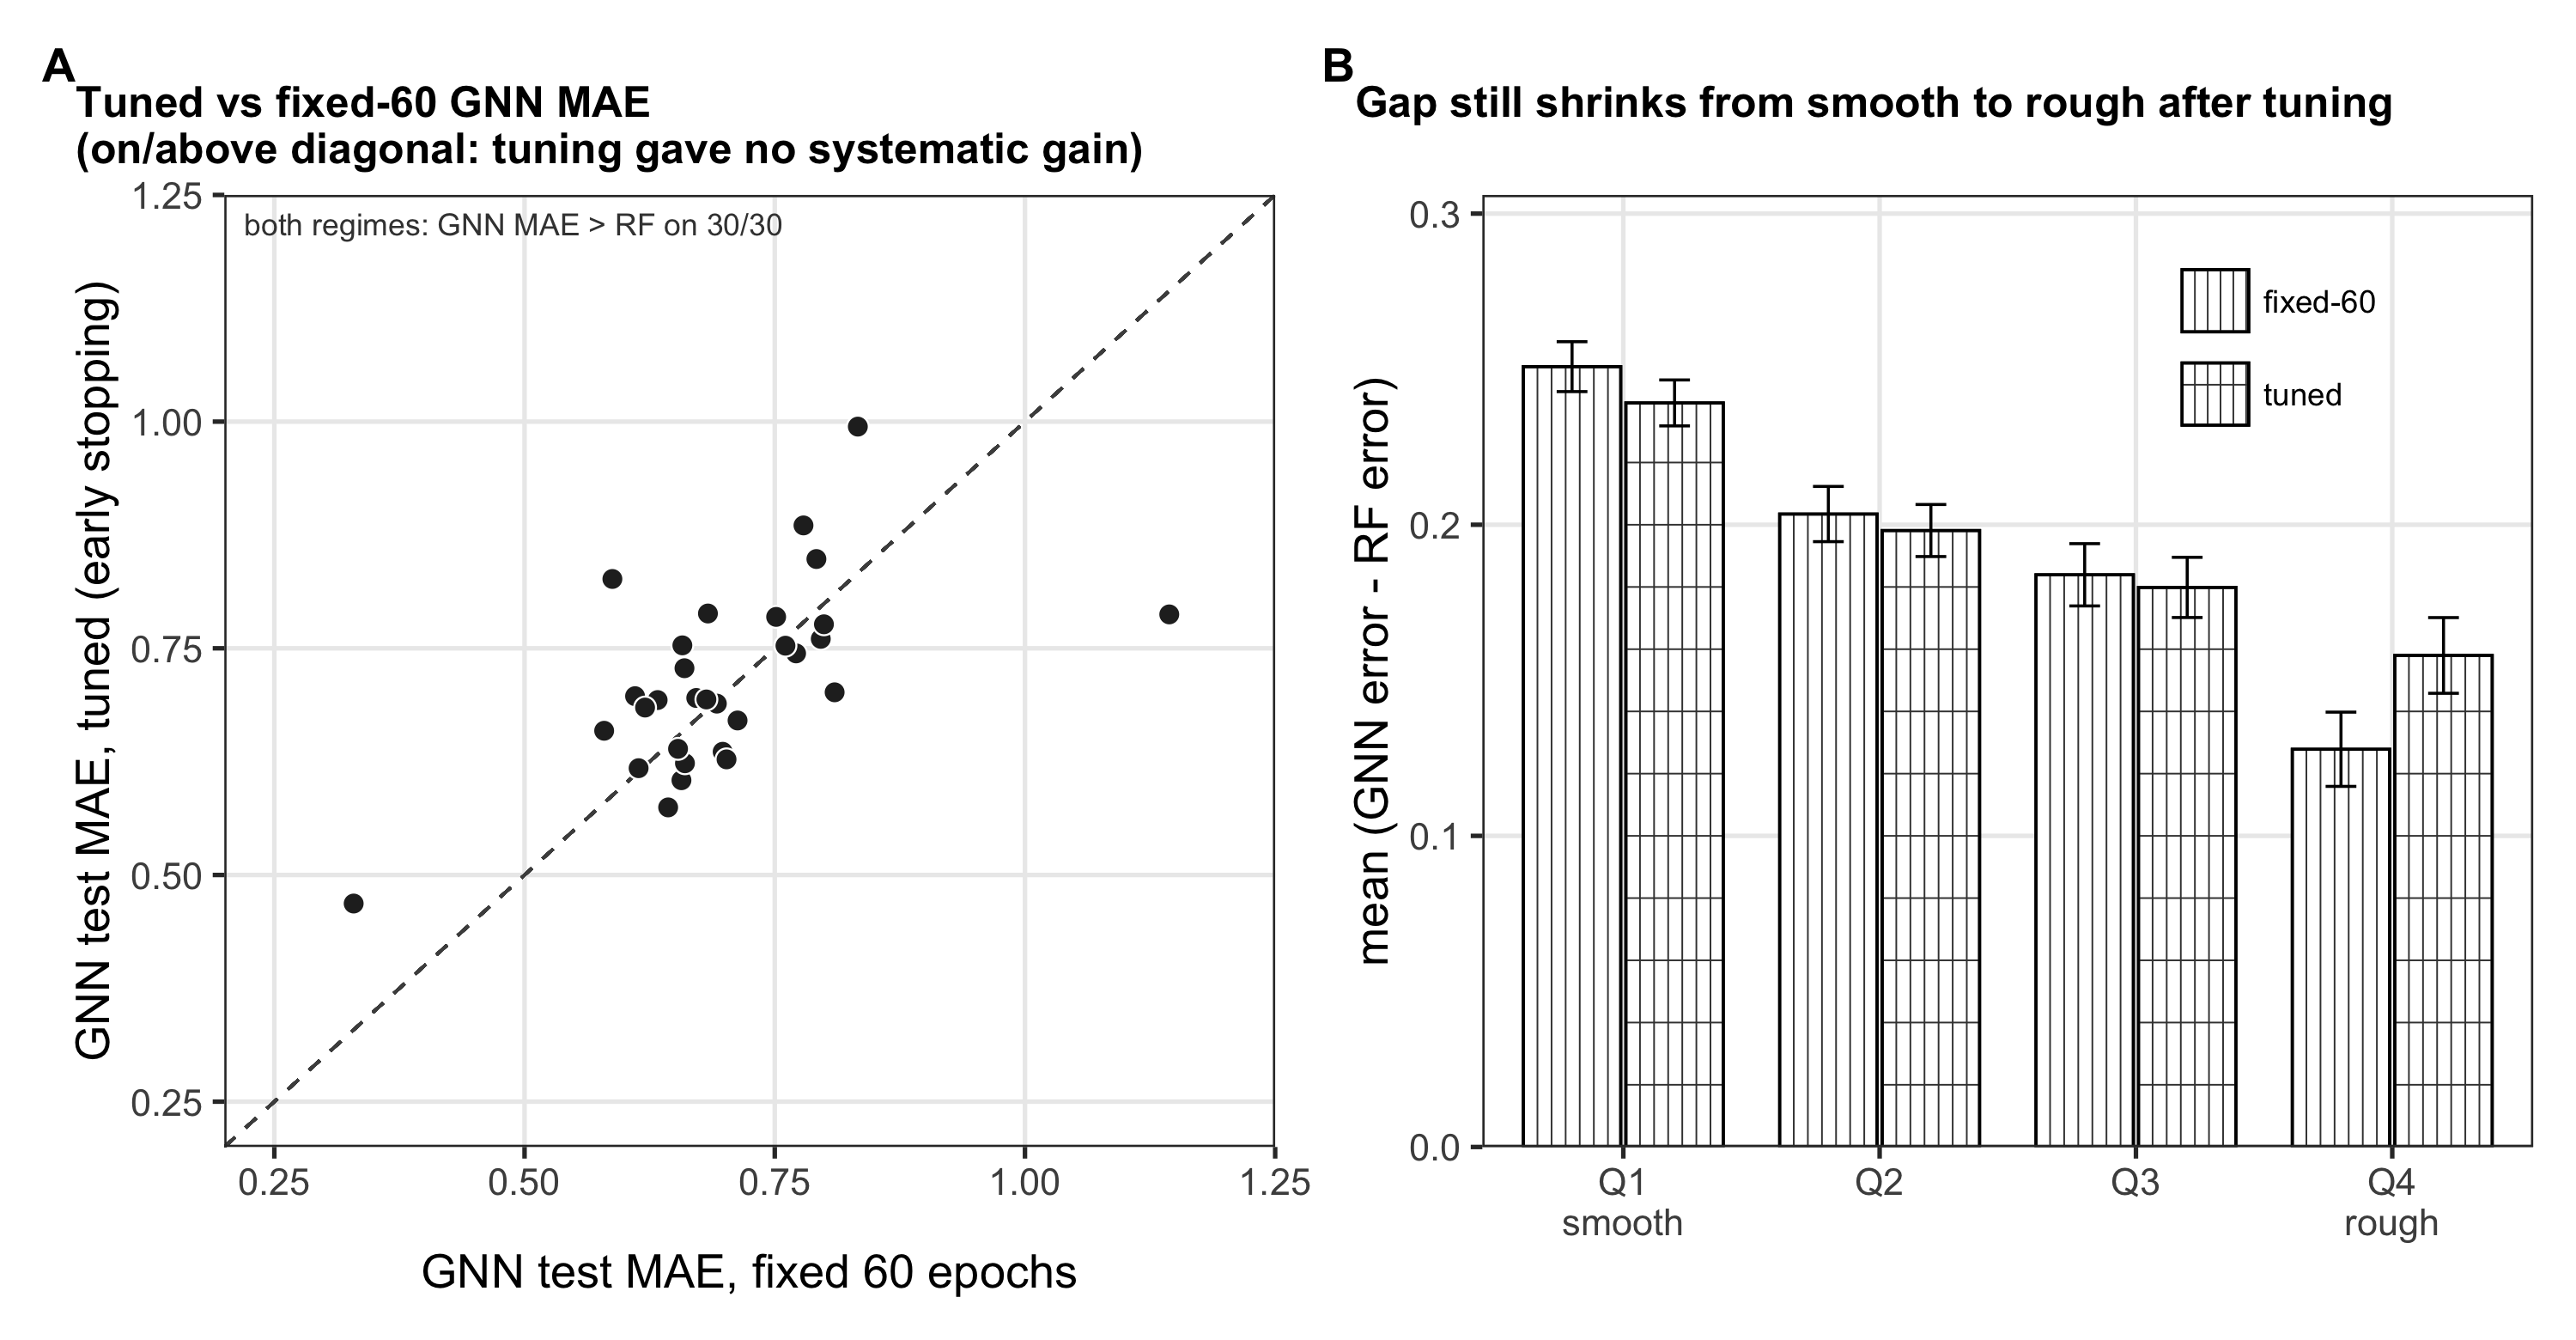
\includegraphics[width=\linewidth]{gnn_tuned_figure.png}
\caption{Comparison with a graph-convolutional baseline. (A) Per-target test mean absolute error of the graph isomorphism network under a fixed 60-epoch schedule versus validated early stopping; both regimens exceed the random-forest error on all 30 targets. (B) Mean (network $-$ random forest) per-compound error by within-target roughness quartile (Q1 smoothest to Q4 roughest) for both regimens; the deficit is largest where the landscape is smooth.}
\label{fig:gnn}
\end{figure}

\subsection*{Local versus global descriptions of landscape roughness}

Finally, we contrasted the per-compound descriptors with a data-set-level description of roughness. The global ROGI index, a single scalar per target, correlated with the fraction of cliff compounds across the 30 benchmarks (Spearman $\rho = 0.60$) but not with the mean random-forest error ($\rho = -0.12$, $p = 0.54$). Two factors plausibly contribute: the benchmarks were curated to be cliff-rich and therefore occupy a narrow band of global roughness (ROGI 0.04--0.11), limiting the variance available to a single scalar, and mean error is additionally governed by data-set size and chemical diversity. Whatever the cause, a global value cannot by construction resolve which compounds within a data set will be mispredicted. The per-compound descriptors developed here address a different and complementary question: not whether a landscape is rough on average, but where on that landscape predictions should be trusted.

\subsection*{Roughness is the right per-compound scale for calibrated intervals}

A conformal predictor turns a point estimate into an interval with a guaranteed coverage rate, but the guarantee is only marginal, and the per-compound variable chosen to make it conditional decides where the coverage actually lands. The conventional choice, the applicability domain, sends it the wrong way. Used as a locally-weighted nonconformity scale, applicability-domain risk drops 90\% interval coverage on labeled activity cliffs to 82.0\%; used as a Mondrian stratifier it leaves coverage falling steadily with local roughness (Figure~\ref{fig:conformal}A), because cliffs are dense rather than sparse and the applicability domain spends interval width in the wrong place. The problem it fails to fix is real. Standard, unconditional intervals reached 90.4\% marginal coverage, but their coverage declined monotonically with local roughness, from 95\% in the smoothest fifth of compounds to 87\% in the roughest (Figure~\ref{fig:conformal}A), and to 87.2\% on labeled cliffs, silently under-covering exactly the compounds a modeler most needs flagged. Conditioning on the activity-free roughness fixes it. A Mondrian predictor stratified by roughness quantile held coverage flat across the entire roughness range, within two points of nominal (Figure~\ref{fig:conformal}A), lifted cliff coverage to 89.5\%, and improved it on 27 of the 30 targets, at a 6\% median increase in interval width (Figure~\ref{fig:conformal}B); a locally-weighted score driven by the same roughness raised cliff coverage to 91.2\%. The contribution is not the normalization, which is standard machinery, but the identification of the right per-compound scale: local roughness makes conformal coverage valid where the landscape is rough, and the applicability domain, which measures distance to the training data, does not.

\begin{figure}[htbp]
\centering
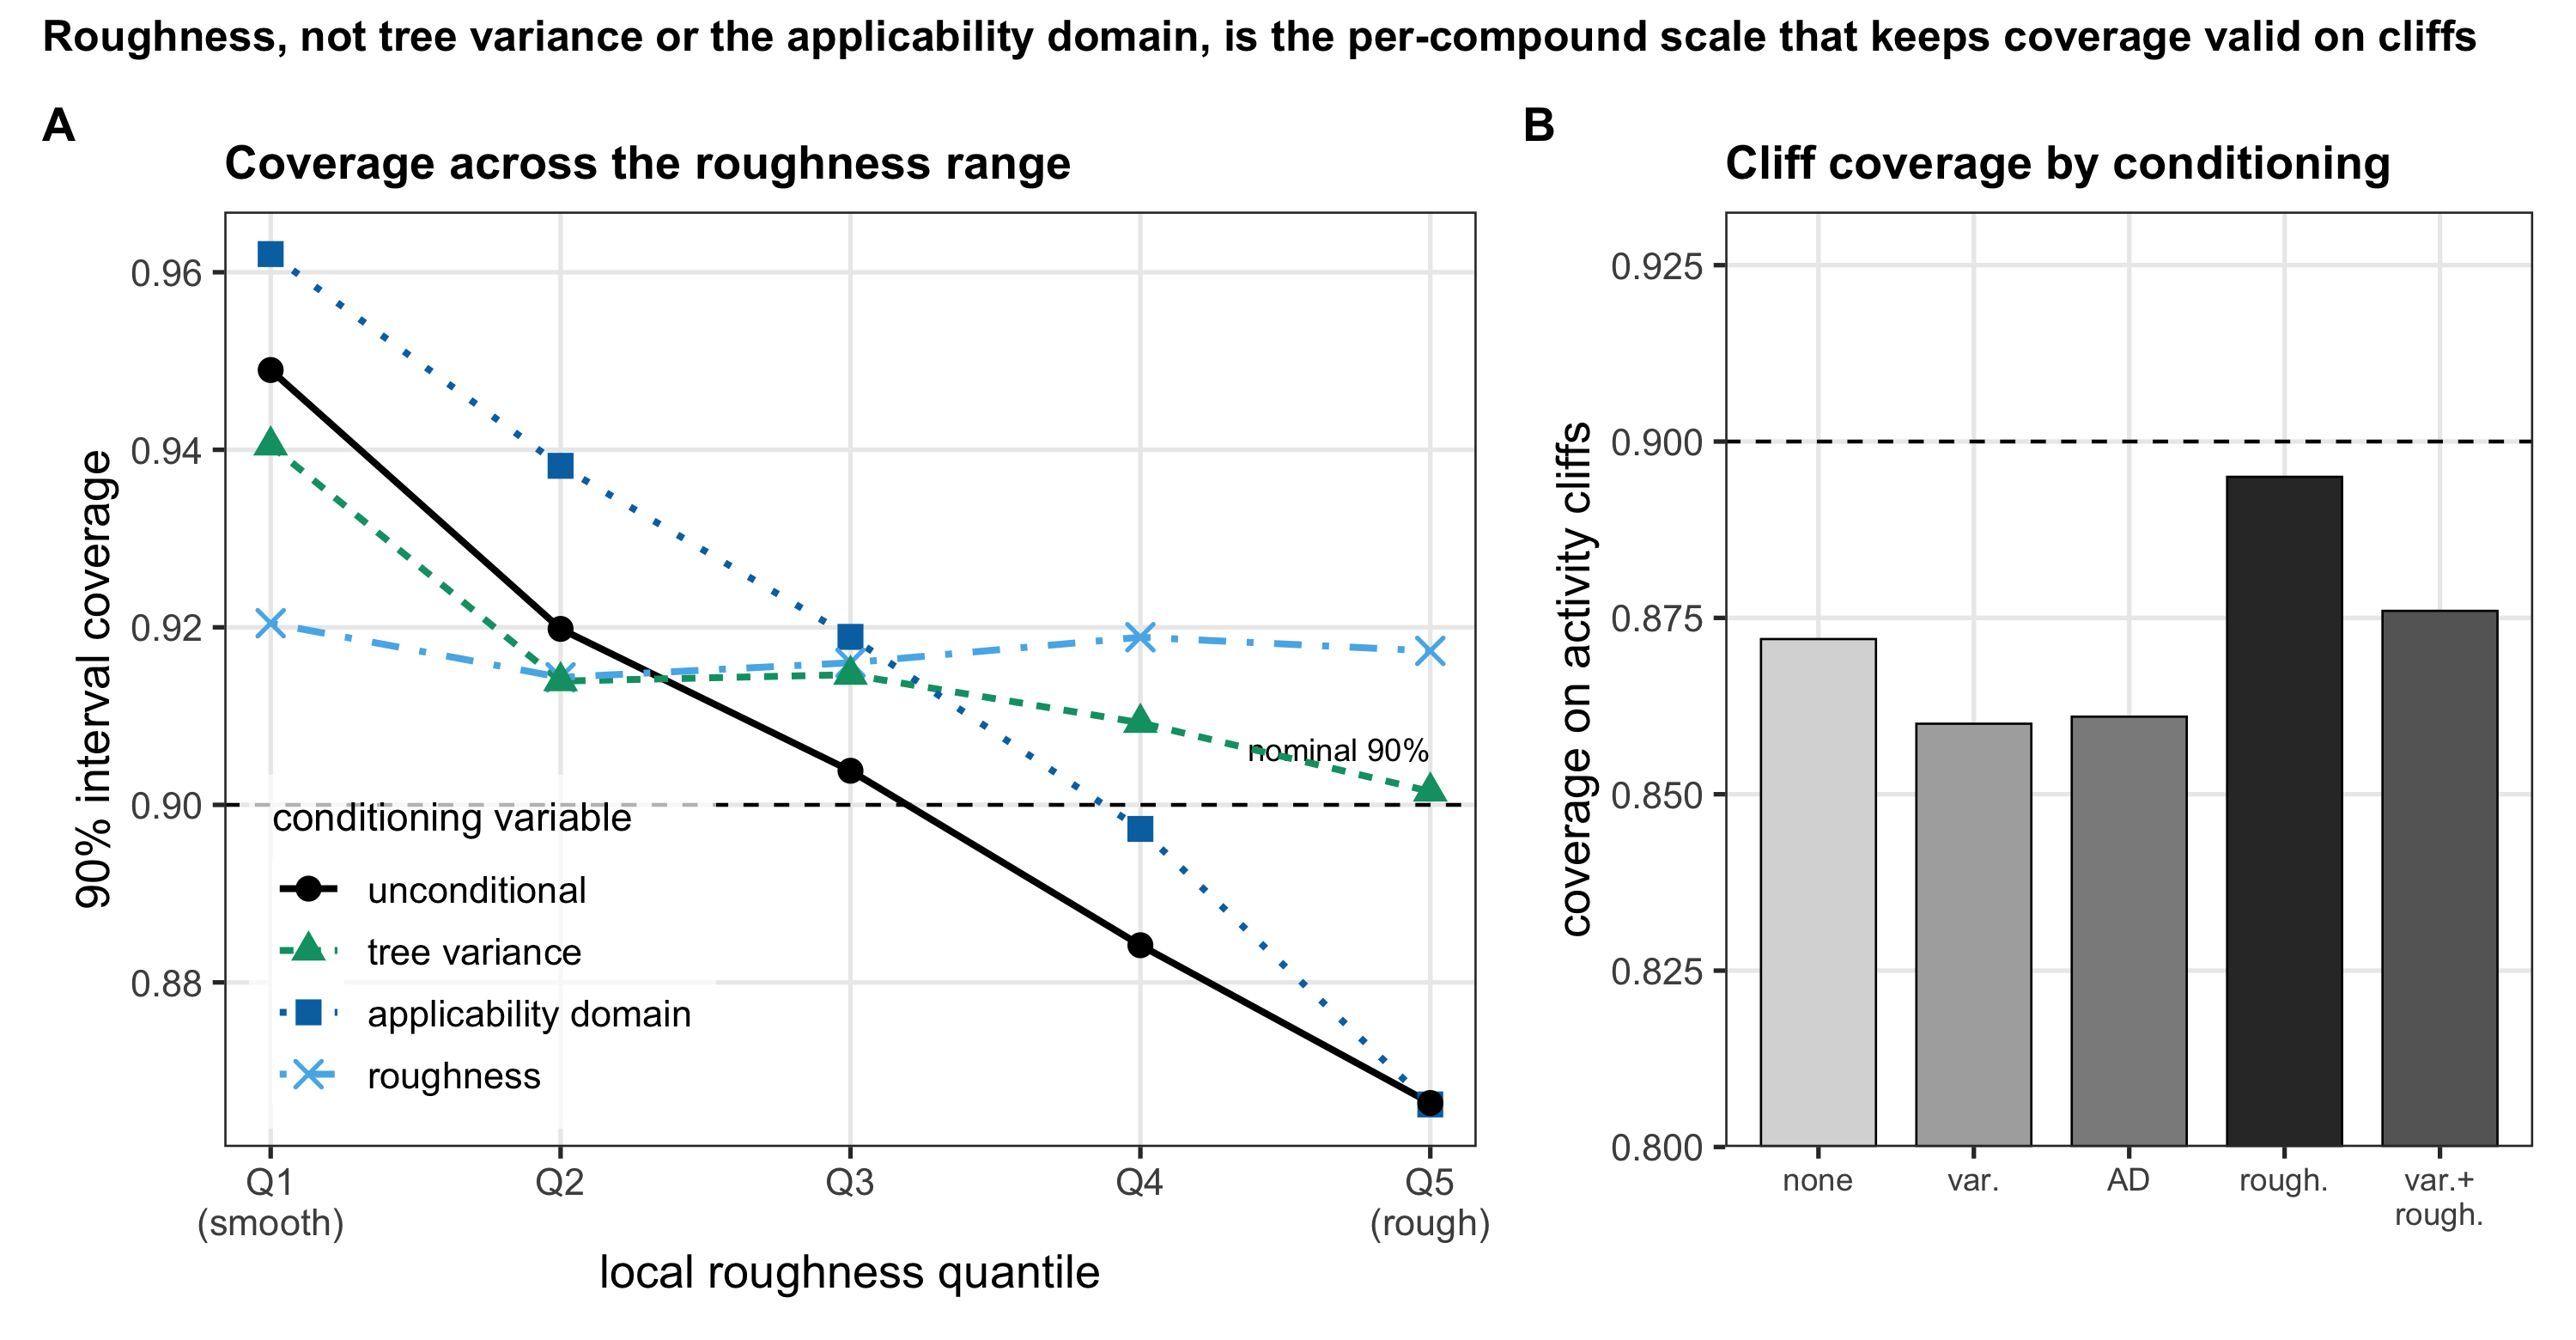
\includegraphics[width=0.92\linewidth]{figure6_conformal.png}
\caption{Roughness-conditioned conformal prediction intervals. (A) Empirical coverage of 90\% inductive-conformal intervals as a function of local-roughness quantile (Q1 smoothest to Q5 roughest), for unconditional (standard) intervals, intervals conditioned on the activity-free roughness, and intervals conditioned on the applicability domain (Mondrian stratification; dashed line, nominal level). Standard coverage declines with roughness and applicability-domain conditioning declines further, whereas roughness conditioning holds coverage flat across the range. (B) Median interval width relative to standard. Median over 30 targets and 50 calibration/evaluation splits.}
\label{fig:conformal}
\end{figure}

\section*{Conclusion}

The error a QSAR model makes on an individual compound is governed substantially by the local roughness of the structure--activity landscape surrounding it, and that roughness can be estimated from chemical structure alone. Across thirty bioactivity benchmarks the relationship was consistent, and it persisted after the applicability domain was controlled, establishing local roughness as a distinct axis of predictability rather than a restatement of distance to the training data. For activity cliffs the two notions are opposed: cliffs concentrate among close structural analogs, the very region in which applicability-domain analysis reports high confidence.

The practical outcome is a per-compound, activity-free reliability estimate. The pairwise-SALI density of a compound's training neighbors flags cliff-prone molecules before any measurement and complements the two reliability signals already in common use, namely distance-based applicability-domain checks (which address extrapolation into sparse chemical space) and ensemble or conformal uncertainty (which address predictive variance), by targeting the dense-region discontinuities that both systematically miss. In a triage setting this distinction is concrete: ranking predictions by roughness preferentially recovers activity cliffs, which ensemble uncertainty flags no better than chance and the applicability domain ranks worse than random; and, used to condition a conformal predictor, the same roughness keeps prediction-interval coverage valid across the roughness range, including on the cliffs where unconditional intervals silently under-cover.

These conclusions are bounded by several limitations. The activity-free effect sizes, although highly consistent across targets, are modest, and the study is confined to bioactivity regression on a single curated benchmark. The graph-convolutional model used to interpret the descriptor-versus-deep-learning gap was not competitive with the descriptor model in absolute terms and was not architecture-optimized, so that comparison is offered only as a supporting observation; and one construct, the local H\"older exponent, did not predict error.

Several directions follow. We found the framework to transfer to physicochemical regression, namely aqueous solubility and lipophilicity (Figure~\ref{fig:crossdomain}), and it should extend further to the quantum-mechanical end points for which large computed data sets exist, where the locality of each property could itself be probed. The conformal demonstration here uses one confidence level and a single conditioning variable; per-target and finer-grained calibration, multi-variable conditioning, and sharper difficulty estimates are natural extensions toward prediction intervals that remain valid wherever the landscape is rough. Stronger activity-free constructs and prospective validation on active discovery campaigns would, finally, test whether structure-only roughness can guide compound triage in practice.

\section*{Associated Content}

\subsection*{Data Availability Statement}

The bioactivity benchmark used in this work (30 ChEMBL targets with activity-cliff annotations and fixed train/test splits) is the publicly available MoleculeACE data set.\cite{vantilborg2022} The external physicochemical benchmarks (ESOL aqueous solubility and Lipophilicity) are distributed publicly with MoleculeNet.\cite{delaney2004,wu2018} All analysis code, the derived per-compound descriptor and error tables, and scripts that regenerate every figure and table in this article are openly available in a public repository (\url{https://github.com/krishnatheaverage/qsar-landscape-roughness}), with a single \texttt{reproduce.sh} entry point and a pinned environment. A frozen snapshot of the repository at the version used for this submission (v1.0.0) is archived on Zenodo (DOI: \texttt{10.5281/zenodo.20603137}). No proprietary or access-restricted data were used.

\subsection*{Supporting Information}

The Supporting Information is available free of charge.
\begin{itemize}
\item Per-target Spearman correlations between each roughness descriptor and per-compound error, applicability-domain partial correlations, and activity-cliff fractions for all 30 benchmark targets; full robustness tables across neighborhood size and molecular distance metric; extended graph-network architecture and training details with per-target errors; conformal prediction-interval coverage by scaling method (PDF)
\end{itemize}

\section*{Author Information}

\noindent\textbf{Corresponding Author}\\
Krishna Harish, Elkins High School, Missouri City, Texas, United States. Email: krishnaharish2009@gmail.com

\noindent\textbf{Notes}\\
The author declares no competing financial interest.

\section*{Funding Sources}

The author received no specific funding for this work.

\section*{Acknowledgements}

The author thanks the developers of RDKit and scikit-learn, and the maintainers of the MoleculeACE and MoleculeNet benchmarks, for making their software and data openly available.

\begin{thebibliography}{99}

\bibitem{vamathevan2019} Vamathevan, J.; Clark, D.; Czodrowski, P.; Dunham, I.; Ferran, E.; Lee, G.; others Applications of Machine Learning in Drug Discovery and Development. \textit{Nat. Rev. Drug Discov.} \textbf{2019}, \textit{18}, 463--477.

\bibitem{walters2021} Walters, W. P.; Barzilay, R. Critical Assessment of AI in Drug Discovery. \textit{Expert Opin. Drug Discov.} \textbf{2021}, \textit{16}, 937--947.

\bibitem{johnson1990} Johnson, M. A.; Maggiora, G. M. \textit{Concepts and Applications of Molecular Similarity}; Wiley: New York, 1990.

\bibitem{maggiora2006} Maggiora, G. M. On Outliers and Activity Cliffs: Why QSAR Often Disappoints. \textit{J. Chem. Inf. Model.} \textbf{2006}, \textit{46}, 1535.

\bibitem{stumpfe2012} Stumpfe, D.; Bajorath, J. Exploring Activity Cliffs in Medicinal Chemistry. \textit{J. Med. Chem.} \textbf{2012}, \textit{55}, 2932--2942.

\bibitem{cruzmonteagudo2014} Cruz-Monteagudo, M.; Medina-Franco, J. L.; P\'erez-Castillo, Y.; Nicolotti, O.; Cordeiro, M. N. D. S.; Borges, F. Activity Cliffs in Drug Discovery: Dr Jekyll or Mr Hyde? \textit{Drug Discov. Today} \textbf{2014}, \textit{19}, 1069--1080.

\bibitem{vantilborg2022} van Tilborg, D.; Alenicheva, A.; Grisoni, F. Exposing the Limitations of Molecular Machine Learning with Activity Cliffs. \textit{J. Chem. Inf. Model.} \textbf{2022}, \textit{62}, 5938--5951. DOI: \texttt{10.1021/acs.jcim.2c01073}.

\bibitem{dablander2023} Dablander, M.; Hanser, T.; Lambiotte, R.; Morris, G. M. Exploring QSAR Models for Activity-Cliff Prediction. \textit{J. Cheminform.} \textbf{2023}, \textit{15}, 47. DOI: \texttt{10.1186/s13321-023-00708-w}.

\bibitem{aldeghi2022} Aldeghi, M.; Graff, D. E.; Frey, N.; Morrone, J. A.; Pyzer-Knapp, E. O.; Jordan, K. E.; Coley, C. W. Roughness of Molecular Property Landscapes and Its Impact on Modellability. \textit{J. Chem. Inf. Model.} \textbf{2022}, \textit{62}, 4660--4671. DOI: \texttt{10.1021/acs.jcim.2c00903}.

\bibitem{graff2023} Graff, D. E.; Pyzer-Knapp, E. O.; Jordan, K. E.; Shakhnovich, E. I.; Coley, C. W. Evaluating the Roughness of Structure--Property Relationships Using Pretrained Molecular Representations. \textit{Digital Discovery} \textbf{2023}, \textit{2}, 1452--1460. DOI: \texttt{10.1039/D3DD00088E}.

\bibitem{golbraikh2014} Golbraikh, A.; Muratov, E.; Fourches, D.; Tropsha, A. Data Set Modelability by QSAR. \textit{J. Chem. Inf. Model.} \textbf{2014}, \textit{54}, 1--4. DOI: \texttt{10.1021/ci400572x}.

\bibitem{peltason2007} Peltason, L.; Bajorath, J. SAR Index: Quantifying the Nature of Structure--Activity Relationships. \textit{J. Med. Chem.} \textbf{2007}, \textit{50}, 5571--5578.

\bibitem{guha2008} Guha, R.; Van Drie, J. H. Structure--Activity Landscape Index: Identifying and Quantifying Activity Cliffs. \textit{J. Chem. Inf. Model.} \textbf{2008}, \textit{48}, 646--658.

\bibitem{netzeva2005} Netzeva, T. I.; Worth, A. P.; Aldenberg, T.; Benigni, R.; Cronin, M. T. D.; Gramatica, P.; others Current Status of Methods for Defining the Applicability Domain of (Quantitative) Structure--Activity Relationships. \textit{ATLA, Altern. Lab. Anim.} \textbf{2005}, \textit{33}, 155--173.

\bibitem{sahigara2012} Sahigara, F.; Mansouri, K.; Ballabio, D.; Mauri, A.; Consonni, V.; Todeschini, R. Comparison of Different Approaches to Define the Applicability Domain of QSAR Models. \textit{Molecules} \textbf{2012}, \textit{17}, 4791--4810.

\bibitem{norinder2014} Norinder, U.; Carlsson, L.; Boyer, S.; Eklund, M. Introducing Conformal Prediction in Predictive Modeling. A Transparent and Flexible Alternative to Applicability Domain Determination. \textit{J. Chem. Inf. Model.} \textbf{2014}, \textit{54}, 1596--1603. DOI: \texttt{10.1021/ci5001168}.

\bibitem{hirschfeld2020} Hirschfeld, L.; Swanson, K.; Yang, K.; Barzilay, R.; Coley, C. W. Uncertainty Quantification Using Neural Networks for Molecular Property Prediction. \textit{J. Chem. Inf. Model.} \textbf{2020}, \textit{60}, 3770--3780. DOI: \texttt{10.1021/acs.jcim.0c00502}.

\bibitem{gaulton2012} Gaulton, A.; Bellis, L. J.; Bento, A. P.; Chambers, J.; Davies, M.; Hersey, A.; others ChEMBL: A Large-Scale Bioactivity Database for Drug Discovery. \textit{Nucleic Acids Res.} \textbf{2012}, \textit{40}, D1100--D1107.

\bibitem{delaney2004} Delaney, J. S. ESOL: Estimating Aqueous Solubility Directly from Molecular Structure. \textit{J. Chem. Inf. Comput. Sci.} \textbf{2004}, \textit{44}, 1000--1005.

\bibitem{wu2018} Wu, Z.; Ramsundar, B.; Feinberg, E. N.; Gomes, J.; Geniesse, C.; Pappu, A. S.; Leswing, K.; Pande, V. MoleculeNet: A Benchmark for Molecular Machine Learning. \textit{Chem. Sci.} \textbf{2018}, \textit{9}, 513--530.

\bibitem{bemis1996} Bemis, G. W.; Murcko, M. A. The Properties of Known Drugs. 1. Molecular Frameworks. \textit{J. Med. Chem.} \textbf{1996}, \textit{39}, 2887--2893.

\bibitem{rogers2010} Rogers, D.; Hahn, M. Extended-Connectivity Fingerprints. \textit{J. Chem. Inf. Model.} \textbf{2010}, \textit{50}, 742--754.

\bibitem{breiman2001} Breiman, L. Random Forests. \textit{Mach. Learn.} \textbf{2001}, \textit{45}, 5--32.

\bibitem{xu2019} Xu, K.; Hu, W.; Leskovec, J.; Jegelka, S. How Powerful Are Graph Neural Networks? International Conference on Learning Representations (ICLR). 2019.

\bibitem{benjamini1995} Benjamini, Y.; Hochberg, Y. Controlling the False Discovery Rate: A Practical and Powerful Approach to Multiple Testing. \textit{J. R. Stat. Soc. B} \textbf{1995}, \textit{57}, 289--300.

\bibitem{papadopoulos2002} Papadopoulos, H.; Proedrou, K.; Vovk, V.; Gammerman, A. Inductive Confidence Machines for Regression. In \textit{Machine Learning: ECML 2002}; Lecture Notes in Computer Science 2430; Springer: Berlin, 2002; pp 345--356.

\bibitem{papadopoulos2011} Papadopoulos, H.; Haralambous, H. Reliable Prediction Intervals with Regression Neural Networks. \textit{Neural Netw.} \textbf{2011}, \textit{24} (8), 842--851.

\bibitem{bostrom2020} Bostr\"om, H.; Johansson, U. Mondrian Conformal Regressors. In \textit{Proceedings of the Ninth Symposium on Conformal and Probabilistic Prediction and Applications}; Proceedings of Machine Learning Research 128; PMLR, 2020; pp 114--133.

\end{thebibliography}

\clearpage
\section*{For Table of Contents Use Only}
\vspace{1em}
\begin{center}
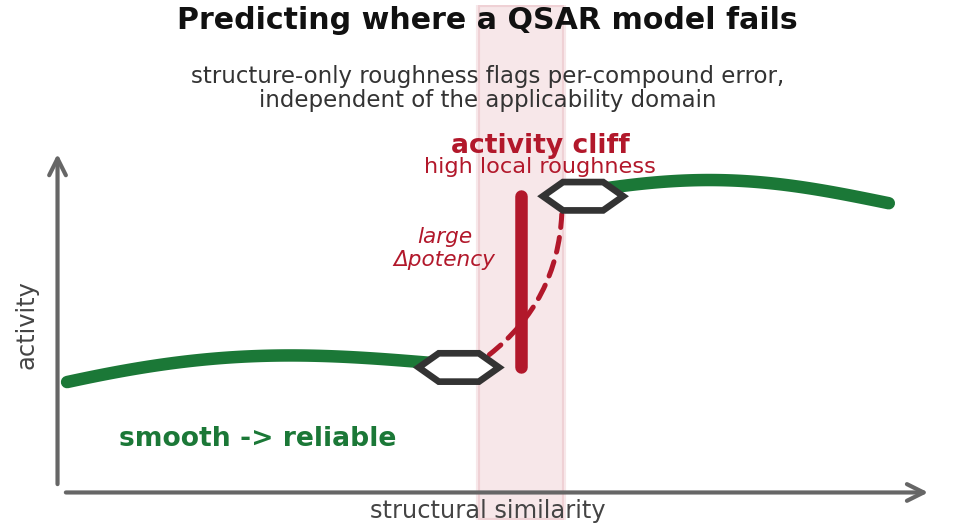
\includegraphics[width=9cm]{TOC_graphic.png}
\end{center}

\end{document}
